\section{Framework}\label{sec:Framework}

\begin{figure}[t]
\centering
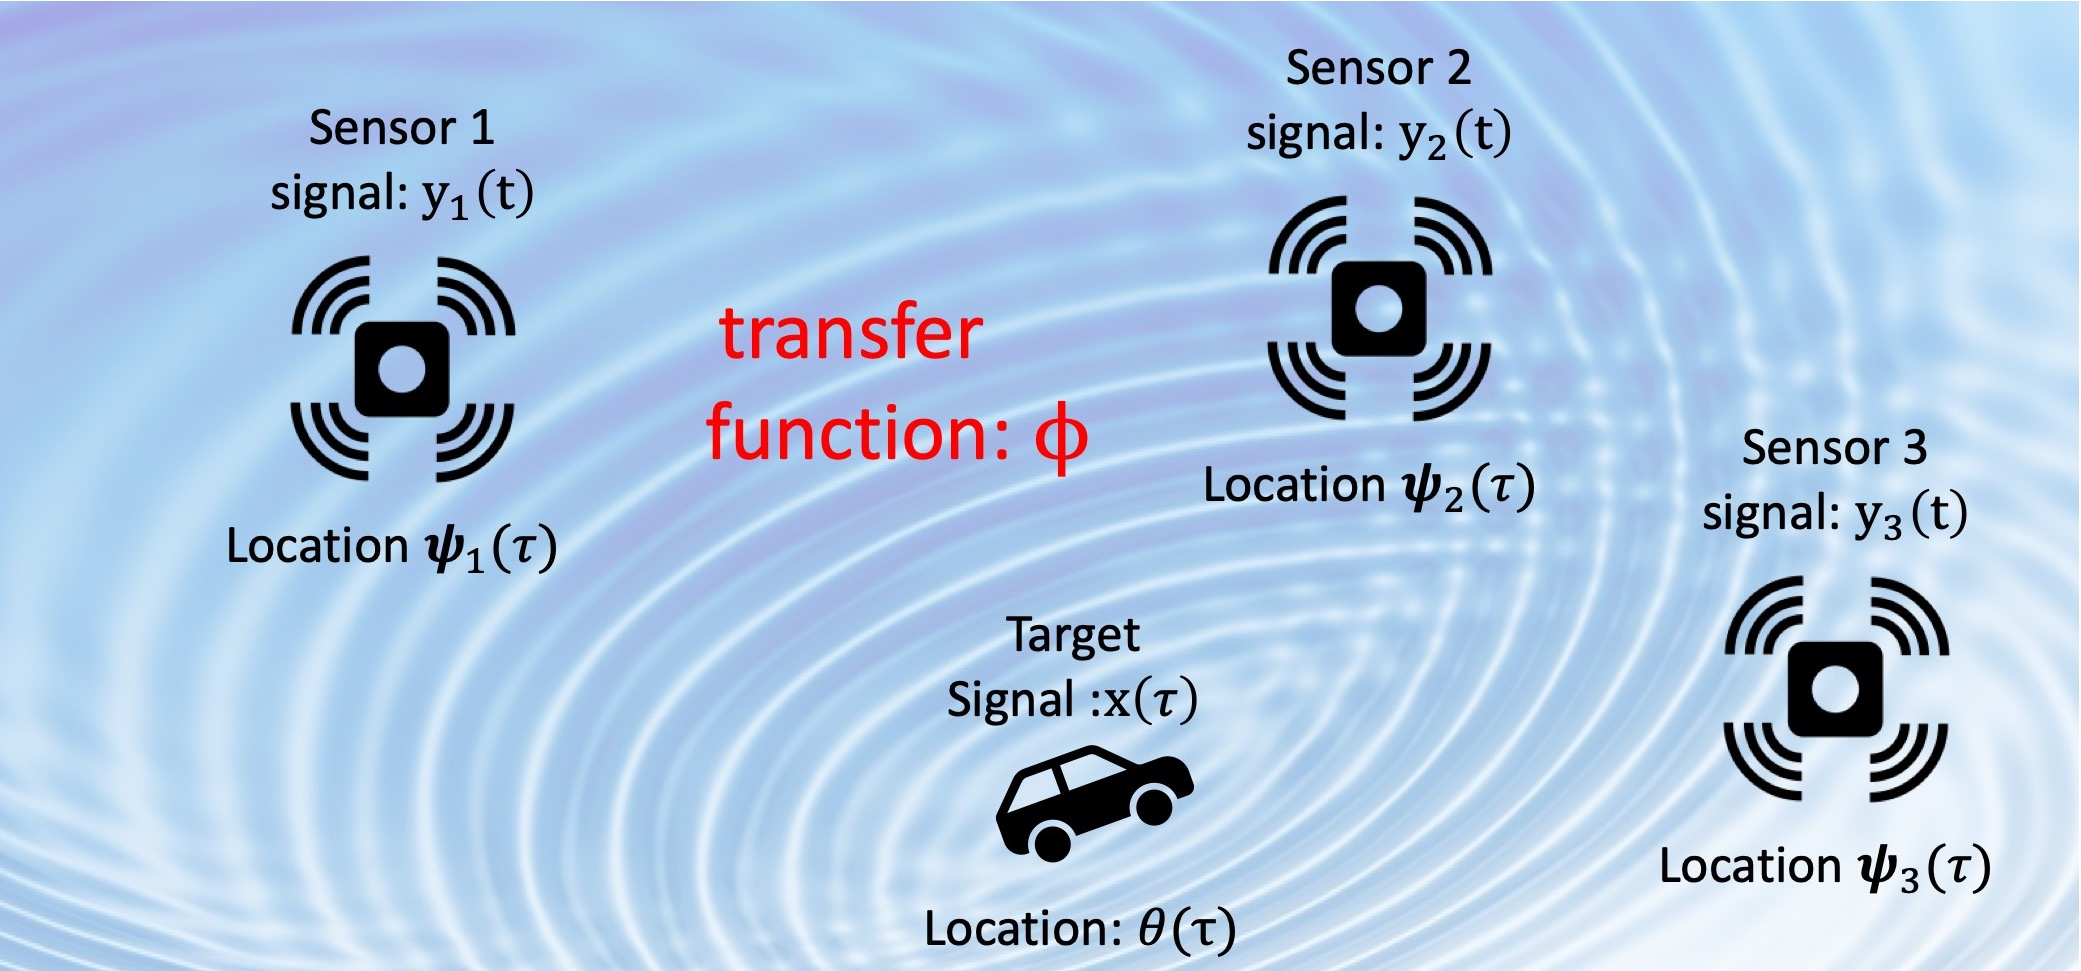
\includegraphics[width=0.7\columnwidth]{figs/Framework.jpg}
\caption{An example of a sensor
  network\label{fig:prototypicalSensorNetwork}. The goal of the
  network is to track a car. The location of the car as a function of
  time is $\theta(\ctime)$, and the goal of the network to produce
  $\estate(\ctime)$. The car emits a sound wave, which we denote by
  $x(\ctime)$. The sound wave travels through the physical environment
  and arrives at $\Sstate_i$ - the location of sensor $i$, where it is digitized and made into a time sequence $y_i(\dtime)$. The transformation of the signal $x(\ctime)$ into $y_i(\dtime)$ is represented by a transfer function $\phi$. In this car tracking example 
$y_i(\dtime) =
\phi(x(\ctime),\state(\ctime),\Sstate_i(\ctime))$
%\rayan{$\psi$ is not  defined here}.
We are seeking an inverse transformation that would map the measurements vector $y_1(\dtime),y_2(\dtime),y_3(\dtime)$ to an estimate of the car location $\estate(\dtime)$}
\end{figure}

This proposal combines several related lines of work. To facilitate the exposition, we start by introducing some terminology and notation that will be used throughout. {\bf Figure~\ref{fig:prototypicalSensorNetwork}} describes a simple sensor network that tracks a car using the sound waves the car is emitting.

We now expand this simple example into a more general framework.
We assume that the network consists of a $n$ sensors and $m$ 
targets. Sensor $i$'s state at time $\ctime$ is denoted $\Sstate_i(\ctime)$.  Similarly, the state of target $j$ at time $\ctime$ is denoted $\state_j(\ctime)$.
Here and in the rest of this section, we don't specify the spaces in which  $\Sstate_i$ or $\state_j$ are members. This allows for a general introduction, and more which will be made more specific in later sections. When appropriate, we will denote the combined state of all targets by $\Vstate(\ctime)$ and the combined state of all sensor by $\VSstate(\ctime)$. The third state component is the state of physical environment in which the targets and sensors reside. We denote the state of the environment by $\env(\ctime)$

The targets generate signals, which we call the {\em raw} signals. We denote the raw signal generated by target $i$ as $\signal_i(\ctime)$. We denote the collection of all $m$ signals by $\Vsignal(\ctime)$. On the receiving end, each sensor $i$ captures a digital signal $\dsignal_i$. These digital signals are the inputs to the computations we will discuss. As the signals arrive at physically separated sensors, the computation is inherently distributed. The main goal of this proposal is to develop algorithms that achieve desired tasks with minimal communication between the sensors.

%\rayan{How are we deciding what variables are in bold and what variables are not? For example, why is $y_i(t)$ not bold in the caption, but $\mathbf{x}_i(\tau)$ in bold?}

The transfer function $\transfer$ defines the way by which the raw signals $\Vsignal$ are transformed into the digitized signals $\Vdsignal$. This function represents both the point transfer function of the physical environment,
the analog-to-digital transformation of the physical signal into a discrete time physical signal, and the noise that is added through this process. The transformation is defined by:\

\begin{equation}
\Vdsignal = \transfer(\Vsignal,\Vstate,\VSstate,\env)\label{eq:transfer}
\end{equation}
Note that the transfer function $\transfer$ operates on the whole sequences, not just on the sequence at a single time $\ctime$. That is because signal propagation takes time, so $\Vdsignal(\dtime)$ depends on $\Vsignal$ at multiple time points.
Many of the problems we plan to tackle in this proposal are inverse
computation problems. We assume that some aspects of the physical
space are known, i.e. we know a subset of
$\Vsignal,\Vstate,\VSstate,\env$. Given the digitized signals
$\Vdsignal$, our task is to estimate the unknown parts of the physical
space. Reliable methods for computing such estimates exist. However,
they typically require high communication bandwidth. The goal of this
proposal is to find distributed estimation algorithms that achieve
good performance while using significantly less communication.

\subsection{Some specific tasks}\label{sec:examples}
We give a few specific examples of tasks. We will elaborate on some of these tasks below
\begin{enumerate}
    \item {\bf Target Localization:}
      Figure~\ref{fig:prototypicalSensorNetwork} depicts an archetypal
      target localization task. In this case the locations of the
      sensors $\VSstate$ and the state of the environment $\env$ are
      assumed to be fixed. A typical additional assumption, which is
      represented in the transfer function $\transfer$, is that
      strongest signal corresponds to the straight line of
      transmission between the target and the sensors. A common
      approach to target localization is to estimate the delay between
      the arrival of the signal at different sensors by using some
      type of cross correlation~\cite{}. This calculation is performed  
      It is well known that placing sensors far from each other
      provides the most accurate localization. However, achieving this
      accuracy with bounded communication between the sensors remains
      a challenge.

    \item{\bf Sensor Calibration:} A common situation is that many sensors
      are installed in an existing environment such as a home, and
      the state of these sensors $\VSstate$ which would typically
      include location and orientation, is not known. Manual
      calibration is often labor intensive or impossible. The
      challenge is to design algorithms through which the network can
      self-calibrate. We consider two types of calibration, in the
      easier {\em active calibration} the system can control the generated
      signals, while in {\em blind calibration} the calibration has to
      be done using signals that are generated by the environment. 

\iffalse      
    \item {\bf Signal reconstruction} Voice based systems such as
      speakerphones, and voice activated computers, need to
      reconstruct the speech signal. Microphone arrays are sensor
      networks where the sensor is a microphone. Accurately
      reproducing the speech signal when there is more than one
      speaker is an open challenge. In this problem the location of
      the sensors is known, the goal is to reproduce the raw signal
      $\Vsignal$. This task is relatively easy when
      $\Vstate,\VSstate,\env$ are known and the transfer function
      $\transfer$ is known and simple. It becomes significantly harder
      when some of $\Vstate,\VSstate,\env$ are unknown or when
      $\transfer$ is complex, such as multi-path radio signals or
      reverberating audio signals.
\fi
    
    \item {\bf Optimizing sensor placement:} The accuracy of target
      localization depends on the location of the target and of the
      sensors. While the location of the target is not under our
      control, the location of the sensors is. Methods for optimizing
      the locations of the sensors will be described in
      Section~{sec:sensor-placement.}
    
    \item{\bf Mapping the environment} Sometime the goal of the system
      is to estimate the environment $\env$. One example is to use
      Radar, Sonar or Lidar to create a 2D or 3D representation of the
      environment for a smart car. Another example, coming from
      seismology is to use controlled vibration sources and many
      acceleration sensors to map the subterranean earth. In these
      settings the locations of the sensors $\VSstate$ and the targets
      $\Vstate$ (called transmitters in this context) is fixed and
      known, as is the raw (transmitted) signal $\Vsignal$. The goal
      is to deduce $\env$ from the collected signal
      $\Vdsignal$. 
    
    \item {\bf Monitoring} \label{item:monitoring} In many situations the goal of the sensor
      network is to track the environment, identify trends and detect
      anomalies. Motivating examples include: Security systems,
      systems for monitoring patients or the elderly, highway
      monitoring and factory floor monitoring. Many of these
      environments are too complex to estimate a fully detailed
      representation. Instead, we suggest building a statistical model
      which implicitly captures the major degrees of freedom of the
      environment and the way they relate to major variables such as
      time of day and day of week.  The challenge here is to learn
      such a model in an unsupervised or weakly supervised way,
      without heavy use of computational or communication
      resources. Here, we will propose, and rigorously analyze
      techniques based on Kernel methods combined with sketching and
      low dimensional binary embedding techniques. The combination of
      these tools will simultaneously facilitate performing various
      desired statistical tasks, while minimizing storage,
      communication, and computational costs.
    
\end{enumerate}

